\documentclass[a4paper,11pt]{scrartcl}

\usepackage[english]{babel}
\usepackage[utf8]{inputenc}
\usepackage[T1]{fontenc}
\usepackage{graphicx}
\usepackage{fullpage}
\usepackage{latexsym}
\usepackage{amssymb}
\usepackage{amsmath}
\usepackage{booktabs}
\usepackage{tabularx}
\usepackage[section]{placeins}
\usepackage{ifthen}
\usepackage{listings}
\usepackage{color}
\usepackage{hyperref}
\usepackage{cite}
\usepackage{csvsimple}
\usepackage{subcaption}
\usepackage{float}

\definecolor{dkgreen}{rgb}{0,0.6,0}
\definecolor{gray}{rgb}{0.5,0.5,0.5}
\definecolor{mauve}{rgb}{0.58,0,0.82}

\lstset{
  language=Python,
  basicstyle=\footnotesize\ttfamily,
  numbers=left,
  numberstyle=\tiny\color{gray},
  stepnumber=1,
  numbersep=5pt,
  backgroundcolor=\color{white},
  showspaces=false,
  showstringspaces=false,
  showtabs=false,
  frame=single,
  rulecolor=\color{black},
  tabsize=4,
  captionpos=b,
  breaklines=true,
  breakatwhitespace=false,
  title=\lstname,
  keywordstyle=\color{blue},
  commentstyle=\color{dkgreen},
  stringstyle=\color{mauve},
  escapeinside={\%*}{*)},
  morekeywords={dataclass,match,case,Self}
}

% Mathematical shortcuts
\newcommand{\N}{\mathbb{N}}
\newcommand{\Z}{\mathbb{Z}}
\newcommand{\R}{\mathbb{R}}
\newcommand{\E}{\mathbb{E}}
\newcommand{\p}{\varphi}
\newcommand{\ta}{\tau}
\newcommand{\la}{\lambda}
\DeclareRobustCommand{\todo}[1]{\textcolor{red}{\textbf{[TO DO: #1]}}}
\addto\captionsenglish{%
  \renewcommand{\lstlistingname}{Code Block}%
  \renewcommand{\lstlistlistingname}{Code Blocks}%
}

\begin{document}

\subject{101.433 Modeling and Simulation (W2026)}
\title{Agent-Based Modeling of Tree Propagation and Seed Dispersal in the city of Vienna}

\publishers{Supervisor: Pernthaner, Hannah}
\author{
    Avakian, Valeriia, \todo{Matriculation number} - \todo{Curriculum number}\footnote{\todo{Fill in once finished}}\\
    Johanna Vaught, Helena, \todo{Matriculation number} - \todo{Curriculum number}\footnote{\todo{Fill in once finished}}\\
    Reyes Polk-Reyes, Mitzalo, 12532869 - \todo{Curriculum number}\footnote{\todo{Fill in once finished}}\\
    Tashkov, Alexander, \todo{Matriculation number} - \todo{Curriculum number}\footnote{\todo{Fill in once finished}}
}

\maketitle

\begin{abstract}
Urban forest dynamics depend strongly on species-specific life-history traits and seed dispersal mechanisms. In this project, we develop a continuous-space, discrete-time agent-based model (ABM) of tree propagation parameterized for urban tree species in Vienna. In the current milestone, we formalize and implement the single-tree reproductive and dispersal subsystem, combining discrete height-class growth, Poisson fecundity, exponential radial dispersal, and an eight-sector directional wind rose. We verify the stochastic dispersal kernel via Monte Carlo simulations and one-sample Kolmogorov--Smirnov goodness-of-fit tests, provide spatial utilities for Vienna's 23 municipal districts, and deliver an interactive Streamlit and Plotly simulation explorer.
\end{abstract}

\newpage

\tableofcontents

\newpage

\section{Introduction}
\paragraph{Motivation.}
Urban forests are ordinarily shaped by active human management, raising the ecological question of how Vienna's tree population would evolve if human intervention ceased entirely. Under a hypothetical scenario in which the city is abandoned and seeds can germinate freely across the urban landscape, regeneration relies solely on sexual reproduction via wind-, animal-, and gravity-mediated dispersal. An agent-based simulation provides a quantitative framework to project how a district's existing street and park trees would drive spontaneous reforestation and determine which species ultimately dominate the future urban canopy.

\paragraph{Introduction to the Topic.}
In agent-based forest models, individual trees occupy continuous spatial coordinates $(x, y) \in \R^2$. Each tree progresses through discrete height classes $k \in \{0, 1, \dots, K\}$, reaches reproductive maturity at species-specific age $A$, and disperses seeds whose radial distances and bearings follow dispersal-mode-specific probability distributions.

\paragraph{Aim.}
The objective of this project is to build a modular, reproducible Python simulation framework for urban tree propagation in Vienna and to analyze the results thereof.

\section{Model}
\subsection{Conceptual Modelling}
\label{sec:modelling}
\paragraph{Agent lifecycle.}
Each tree agent $i$ is represented with integer age $a_i \in \N_0$, discrete height class $k_i \in \{0, 1, \dots, K\}$, and status $\text{ALIVE}$ or $\text{DEAD}$. Given a species' years per height class $T \in \N_{>0}$ and maximal height class $K \in \N_{>0}$, the height class at age $a_i$ is defined deterministically as
\begin{equation}
\label{eq:height_class}
k(a_i) = \min\!\left(K, \left\lfloor \frac{a_i}{T} \right\rfloor \right).
\end{equation}
When initializing an agent solely from a known height class $k_i$, its baseline age is estimated as $a_{\text{est}} = k_i \cdot T$.

\todo{Describe mortality when implemented.}

\paragraph{Agent positioning.}
Each tree agent $i$ is represented at an exact metric position $(x_i, y_i) \in \R^2$ (with $+x$ pointing East and $+y$ pointing North), which is then mapped onto a grid of cells of a given edge length $\Delta$.

\todo{Describe x,y mapping to grid coords when implemented.}

\paragraph{Seed Production.}
A tree produces seeds only once it has reached reproductive maturity ($a_i \ge A$). For each species the height-adjusted expected seed output is $\la_i = \p \cdot k_i$ where $\p$ is the species fecundity, and the actual annual seed count $N_{\text{seeds}, i}$ is drawn from a Poisson distribution:
\begin{equation}
\label{eq:fecundity}
N_{\text{seeds}, i} \sim
\begin{cases}
\text{Poisson}(\p \cdot k_i), & \text{if } a_i \ge A \text{ and } k_i > 0, \\
0, & \text{otherwise.}
\end{cases}
\end{equation}

\paragraph{Dispersal Kernel and Directional Bearings.}
Each produced seed $j \in \{1, \dots, N_{\text{seeds}, i}\}$ is dispersed independently from the parent's exact coordinates $(x_i, y_i)$. Its radial dispersal distance $R_j$ follows an exponential distribution $R_j \sim \text{Exp}(\bar{r})$ with probability density function
\begin{equation}
\label{eq:exp_pdf}
f_R(r) = \frac{1}{\bar{r}} \exp\!\left(-\frac{r}{\bar{r}}\right), \qquad r \ge 0,
\end{equation}
where the theoretical mean dispersal radius $\bar{r}$ depends on the species' dispersal mode, wind strength $s \in \N_{>0}$, wind spreading factor $f > 0$, or fixed animal/gravity mean dispersal distance $d_m > 0$:
\begin{equation}
\label{eq:mean_radius}
\bar{r} =
\begin{cases}
s \cdot f \cdot k_i, & \text{if dispersal mode is \texttt{wind}}, \\
d_m, & \text{if dispersal mode is \texttt{animal} or \texttt{gravity}}.
\end{cases}
\end{equation}

Travel bearings $\theta_j \in [0, 2\pi)$ are measured clockwise from North. For \texttt{animal} and \texttt{gravity} dispersal, bearings are isotropic: $\theta_j \sim \mathcal{U}(0, 2\pi)$. For \texttt{wind} dispersal, an incoming wind sector $c \in \{\text{N}, \text{NE}, \text{E}, \text{SE}, \text{S}, \text{SW}, \text{W}, \text{NW}\}$ (with sector centers $\mu_c \in \{0^\circ, 45^\circ, \dots, 315^\circ\}$) is sampled according to the wind rose probabilities $p_c$ ($\sum_c p_c = 1$), which are then perturbed uniformly within the $45^\circ$ sector, and rotated $180^\circ$ downwind:
\begin{equation}
\label{eq:wind_bearing}
\theta_j = \frac{\pi}{180} \Big( (\mu_c + \varepsilon_j + 180^\circ) \bmod 360^\circ \Big), \qquad \varepsilon_j \sim \mathcal{U}(-22.5^\circ, 22.5^\circ).
\end{equation}
The seed's landing coordinates $(x_{\text{land}, j}, y_{\text{land}, j})$ are then given by
\begin{equation}
\label{eq:landing_coords}
\begin{pmatrix} x_{\text{land}, j} \\ y_{\text{land}, j} \end{pmatrix}
=
\begin{pmatrix} x_i \\ y_i \end{pmatrix}
+ R_j
\begin{pmatrix} \sin \theta_j \\ \cos \theta_j \end{pmatrix}.
\end{equation}


\subsection{Parametrisation}
\label{sec:parametrisation}

Species parameters are loaded from \texttt{data/tree\_species\_config.csv} and validated against specific constraints. Table~\ref{tab:species_schema} summarizes the parameter schema and domain constraints enforced by the codebase, while Table~\ref{tab:env_defaults} lists the default environmental, wind-rose, and simulation parameters.

\begin{table}[!ht]
\centering
\small
\begin{tabularx}{\textwidth}{l l l >{\raggedright\arraybackslash}X}
\toprule
\textbf{CSV Column} & \textbf{Model Symbol} & \textbf{Domain / Constraint} & \textbf{Description} \\
\midrule
\texttt{species} & --- & Non-empty string & Unique tree species name \\
\texttt{dispersal} & --- & $\{\texttt{wind}, \texttt{animal}, \texttt{gravity}\}$ & Seed dispersal mechanism \\
\texttt{f} & $f$ & $f > 0$ (for \texttt{wind}) & Wind spreading factor [m] \\
\texttt{d\_m} & $d_m$ & $d_m > 0$ (for \texttt{animal}, \texttt{gravity}) & Mean dispersal distance [m] \\
\texttt{phi} & $\p$ & $\p \ge 0$ & Baseline fecundity [seeds / (yr $\cdot$ height class)] \\
\texttt{A\_yr} & $A$ & $A \in \N_0$, $A < L$ & Reproductive maturity age [yr] \\
\texttt{T\_yr} & $T$ & $T \in \N_{>0}$ & Years required per height class [yr] \\
\texttt{K} & $K$ & $K \in \N_{>0}$ & Maximal discrete height class \\
\texttt{L\_yr} & $L$ & $L \in \N_{>0}$, $L > A$ & Mean lifespan [yr] \\
\texttt{tau} & $\ta$ & $\ta \in [0, 1]$ & Shade tolerance index \\
\bottomrule
\end{tabularx}
\caption{Species trait schema.}
\label{tab:species_schema}
\end{table}

\begin{table}[!ht]
\centering
\footnotesize
\setlength{\tabcolsep}{5pt}
\begin{tabular}{l l l}
\toprule
\textbf{Parameter} & \textbf{Default Value} & \textbf{CONST} \\
\midrule
Default random seed & $10$ & \texttt{DEFAULT\_RANDOM\_SEED} \\
Default height class $k$ & $4$ & \texttt{DEFAULT\_HEIGHT\_CLASS} \\
Default wind strength $s$ & $10$ & \texttt{DEFAULT\_WIND\_STRENGTH} \\
MC instances & & \\
\hspace{1.2em}Seed dispersal & $1000$ & \texttt{DEFAULT\_SEED\_DISPERSAL\_SIMULATION\_INSTANCES} \\
\hspace{1.2em}\todo{add if relevant} & \todo{add if relevant} & \todo{add if relevant} \\
Default wind rose & $(0.06, 0.05, 0.06, 0.18, 0.07, 0.06, 0.30, 0.22)$ & \texttt{DEFAULT\_WIND\_ROSE} \\
\todo{add if relevant} & \todo{add if relevant} & \todo{add if relevant} \\
\bottomrule
\end{tabular}
\caption{Default environment, simulation, and geospatial configuration values.}
\label{tab:env_defaults}
\end{table}

\FloatBarrier
\subsection{Implementation}
\label{sec:implementation}

The codebase is organized as a modular Python package (\texttt{src/tree\_propagation/}) paired with an interactive Streamlit dashboard (\texttt{app.py}) and auxiliary analytics notebooks:
\begin{itemize}
    \item \textbf{Core Domain:} \todo{Describe agents, grids and configurations code structure}. 
    
    Code Block~\ref{src:snip1} illustrates placeholder functionality from 

    \texttt{src/tree\_propagation/PLACEHOLDER.py}.
    \item \textbf{Simulations:} \todo{Describe simulation code structure.}
    
    Code Block~\ref{src:snip2} illustrates placeholder functionality from 

    \texttt{src/tree\_propagation/PLACEHOLDER.py}.
    \item \textbf{Metrics:} \todo{Describe metrics code structure.}
    
    Code Block~\ref{src:snip3} illustrates placeholder functionality from 

    \texttt{src/tree\_propagation/PLACEHOLDER.py}.
    \item \textbf{Visualization:} \todo{Describe visualization code structure.}
    
    Code Block~\ref{src:snip4} illustrates placeholder functionality from 

    \texttt{src/tree\_propagation/visualization/PLACEHOLDER.py}.
    \item \textbf{App:} \todo{Describe app structure.}

    Code Block~\ref{src:snip5} illustrates placeholder functionality from 
    \texttt{app.py}.
\end{itemize}

\begin{lstlisting}[
  caption={PLACEHOLDER snippet 1},
  label={src:snip1}
]
print("Hello world!")
\end{lstlisting}

\begin{lstlisting}[
  caption={PLACEHOLDER snippet 2},
  label={src:snip2}
]
print("Hello world!")
\end{lstlisting}

\begin{lstlisting}[
  caption={PLACEHOLDER snippet 3},
  label={src:snip3}
]
print("Hello world!")
\end{lstlisting}

\begin{lstlisting}[
  caption={PLACEHOLDER snippet 4},
  label={src:snip4}
]
print("Hello world!")
\end{lstlisting}

\begin{lstlisting}[
  caption={PLACEHOLDER snippet 5},
  label={src:snip5}
]
print("Hello world!")
\end{lstlisting}

\section{Simulation Results}

In order to guarantee reproducibility, for all stochastic processes we use the default seed from (Table~\ref{fig:wind_rose})

\subsection{Species seed shadow simulation}
We evaluated the seed shadows for a single tree of each species under Vienna's wind rose (Figure~\ref{fig:wind_rose}) at default wind strength $s = 10$ and height class $k = 4$ over $N = 1000$ simulations.

\begin{figure}[!ht]
 \centering
 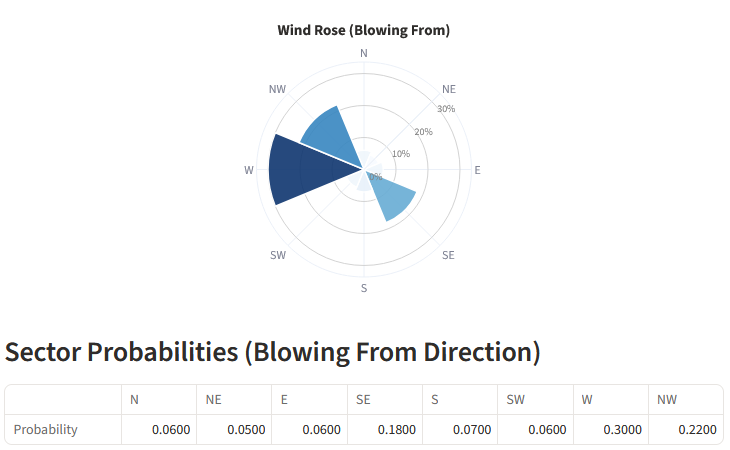
\includegraphics[width=\textwidth]{./images/wind_rose.png}
 \caption{Wind rose indicates where the wind blows \textit{from} and with what probability. Seeds are then dispersed in the opposite direction.}
 \label{fig:wind_rose}
\end{figure}

\begin{itemize}
    \item \textbf{Spatial Anisotropy vs. Isotropy:} Wind-dispersed species exhibit pronounced downwind elongation toward the East and Southeast (opposite the dominant W/NW sectors), whereas gravity- and animal-dispersed species form radially symmetric seed shadows centered at $(0, 0)$.
    \item \textbf{Distributional Verification:} As the number of Monte Carlo ensembles increases, the empirical mean dispersal radius converges closely to the analytical expectation $\bar{r}$ (Equation~\ref{eq:mean_radius}), and the one-sample Kolmogorov--Smirnov test consistently fails to reject the null hypothesis $R \sim \text{Exp}(\bar{r})$ ($p > 0.05$).
\end{itemize}

\begin{table}[H]
  \centering
  \small
  \csvreader[
    tabular=llrrrrr,
    table head=\toprule
      \textbf{Species} &
      \textbf{Dispersal} &
      \textbf{Total Seeds} &
      $\bar{r}_{\text{theory}}$ \textbf{[m]} &
      $\bar{r}_{\text{sim}}$ \textbf{[m]} &
      \textbf{Rel. Error [\%]} &
      \textbf{KS $p$-value} \\ \midrule,
    table foot=\bottomrule,
    late after line=\\
  ]{./tables/seed_dispersal_montecarlo_results.csv}{}{%
    \csvcoli & \csvcolii & \csvcoliii & \csvcoliv & \csvcolv & \csvcolvi & \csvcolvii
  }
  \caption{Monte Carlo seed-dispersal verification results across species ($s = 10$, $k = 4$, $N = 1000$).}
  \label{tab:seed_dispersal_mc}
\end{table}

\clearpage
\begin{figure}[H]
    \centering
    \begin{subfigure}[b]{0.49\textwidth}
        \centering
        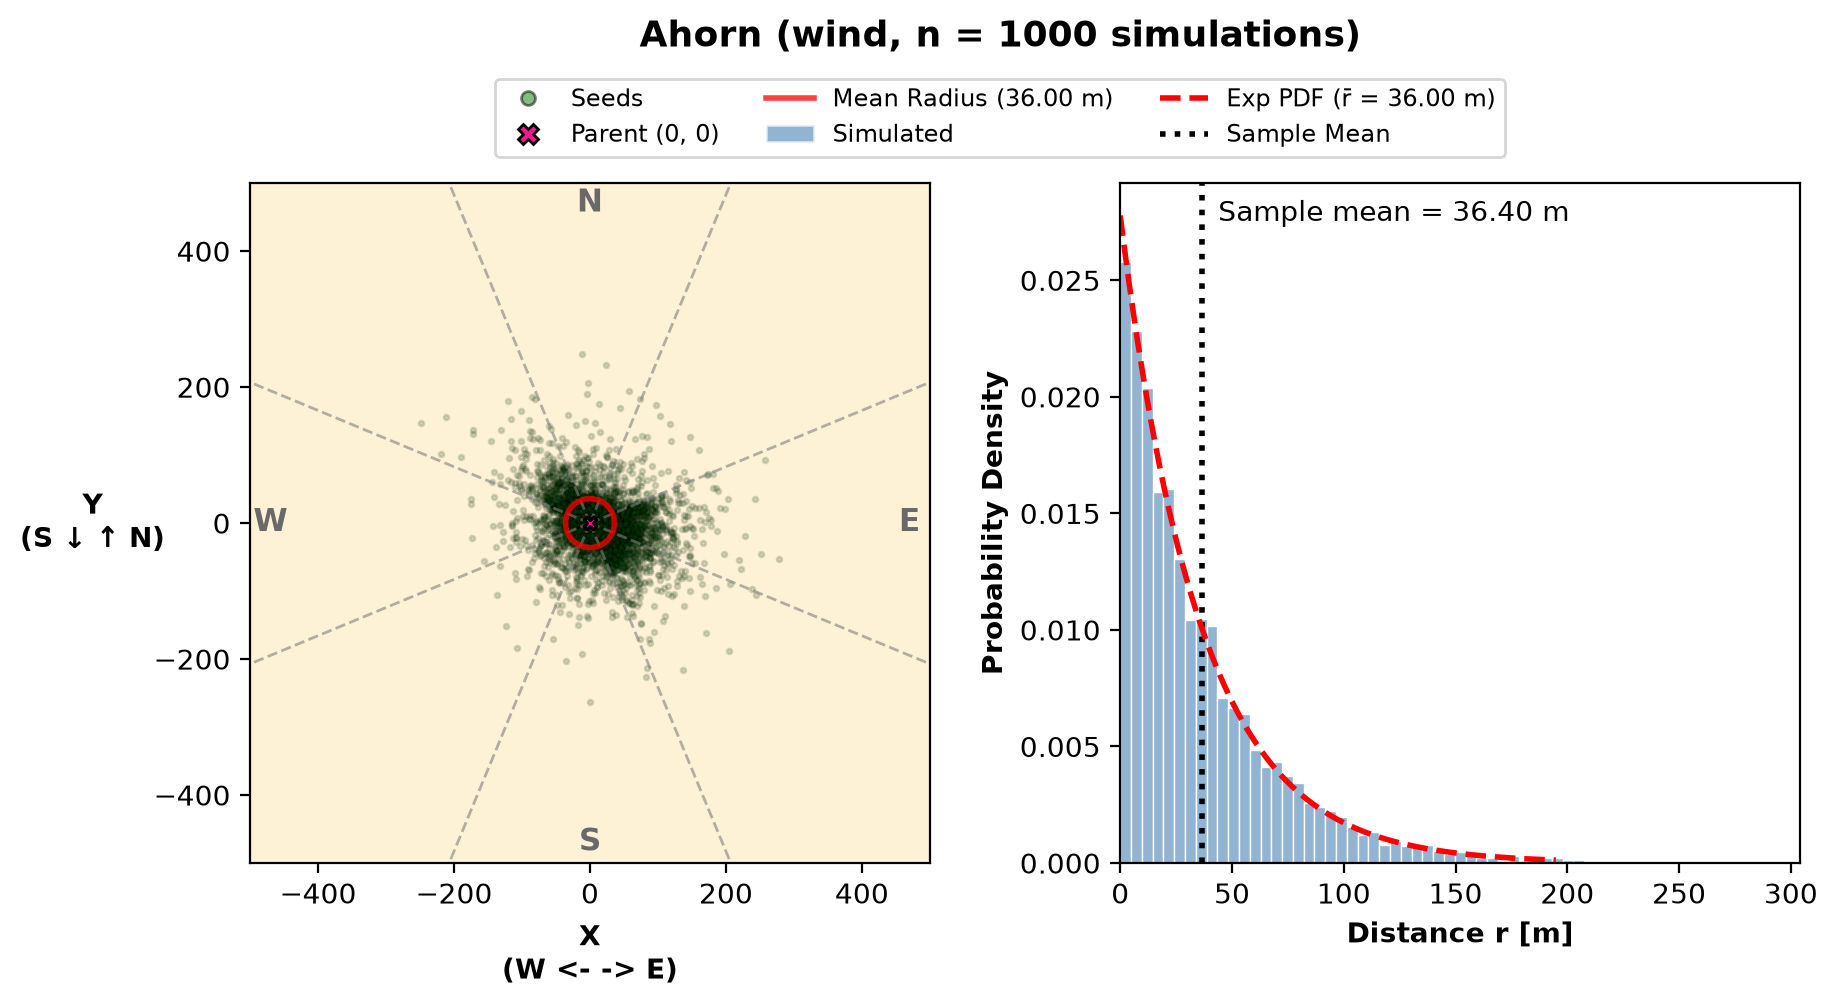
\includegraphics[width=\linewidth]{images/seed_shadow_Ahorn.png}
        \caption{Ahorn (wind)}
        \label{fig:seed_shadow_ahorn}
    \end{subfigure}\hfill
    \begin{subfigure}[b]{0.49\textwidth}
        \centering
        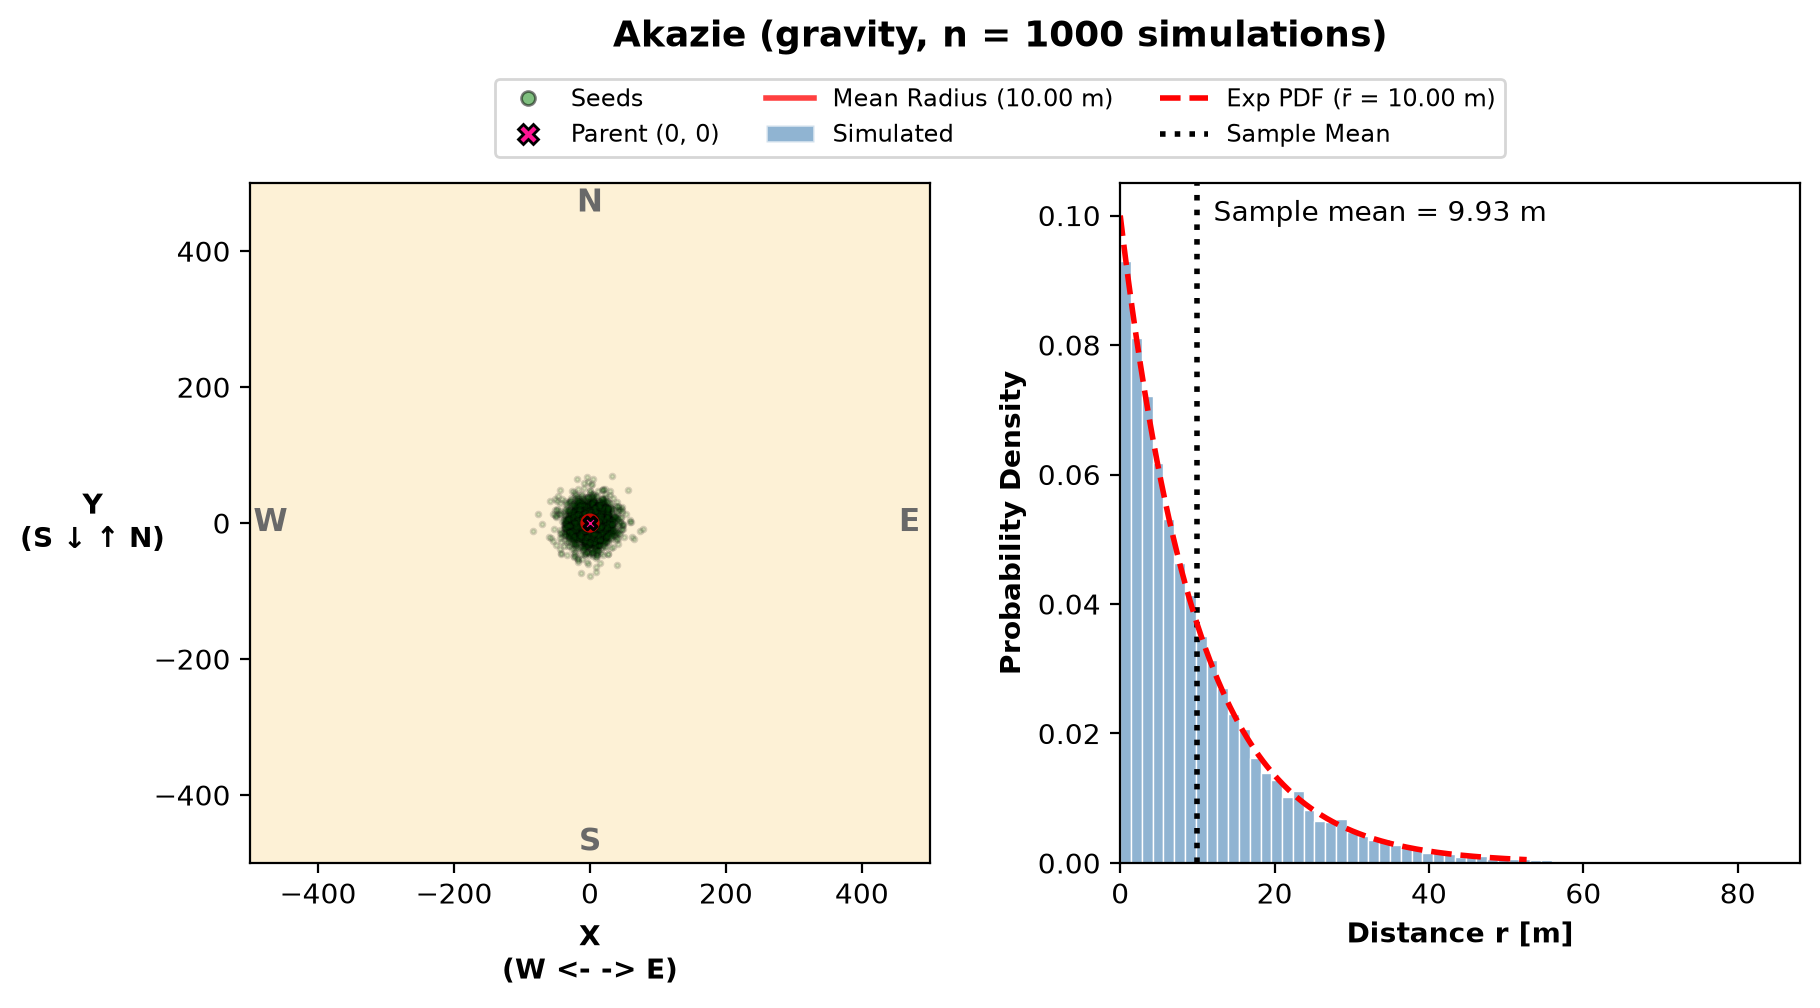
\includegraphics[width=\linewidth]{images/seed_shadow_Akazie.png}
        \caption{Akazie (gravity)}
        \label{fig:seed_shadow_akazie}
    \end{subfigure}

    \vspace{0.6em}
    \begin{subfigure}[b]{0.49\textwidth}
        \centering
        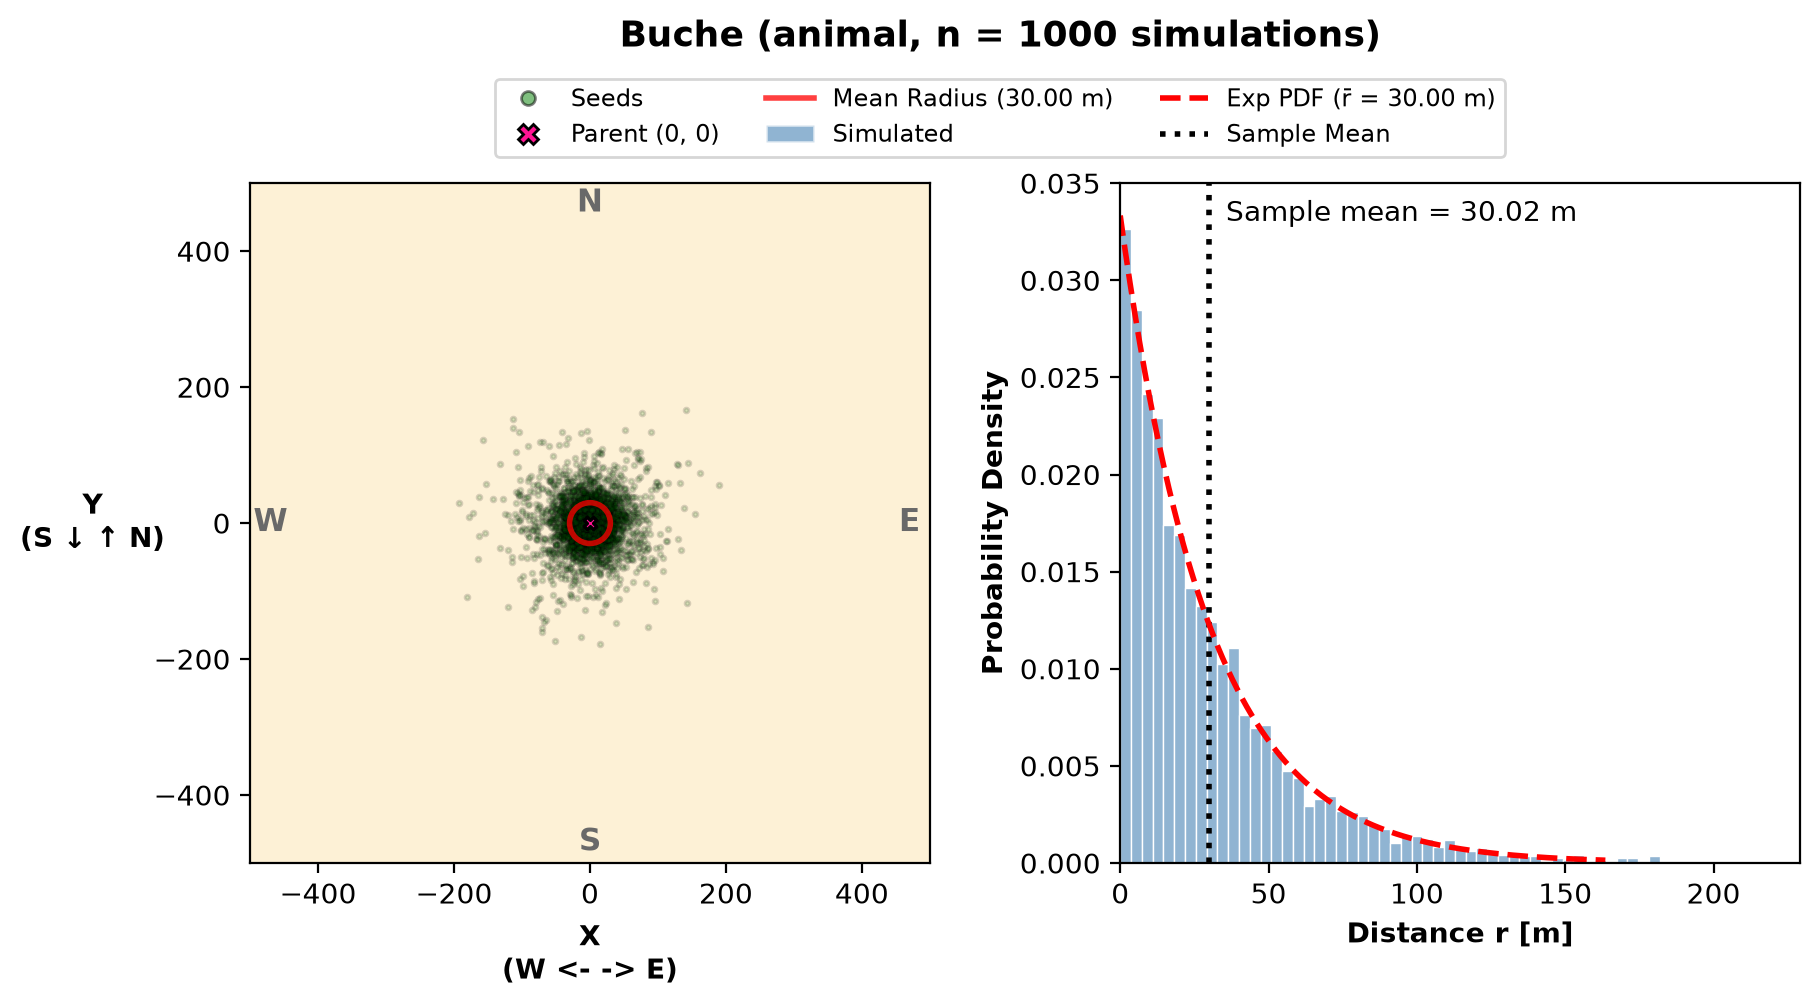
\includegraphics[width=\linewidth]{images/seed_shadow_Buche.png}
        \caption{Buche (animal)}
        \label{fig:seed_shadow_buche}
    \end{subfigure}\hfill
    \begin{subfigure}[b]{0.49\textwidth}
        \centering
        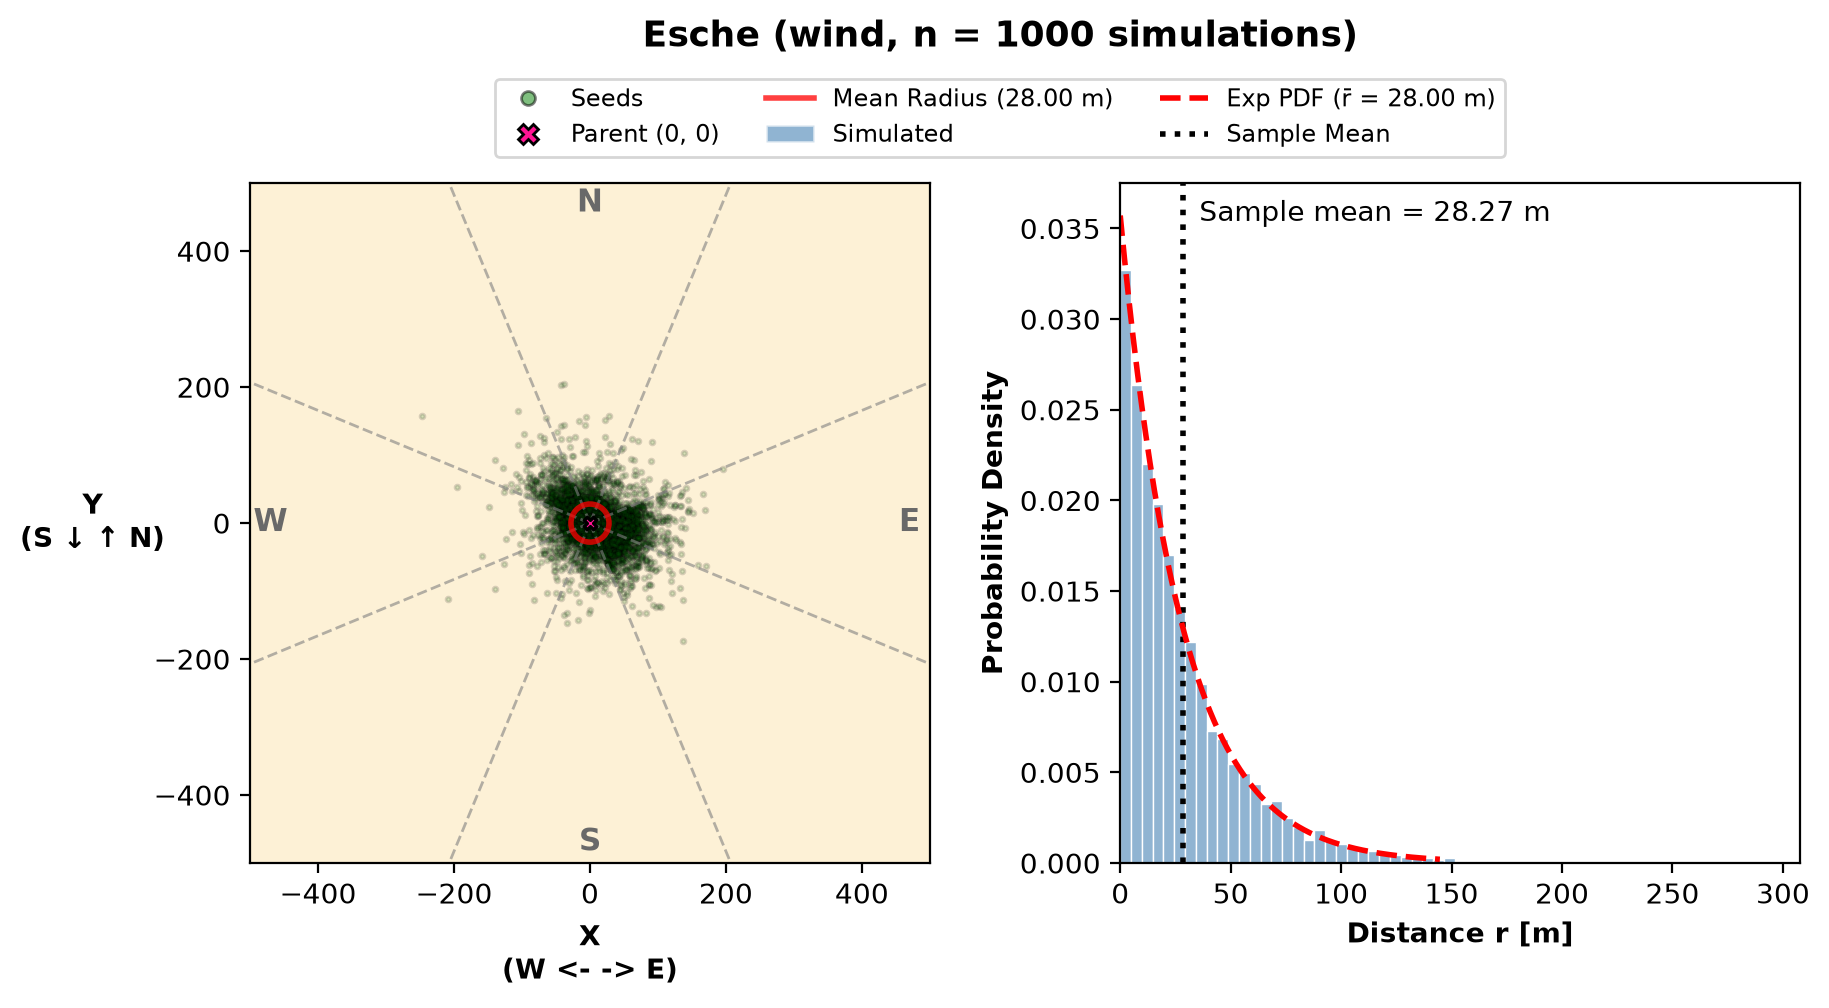
\includegraphics[width=\linewidth]{images/seed_shadow_Esche.png}
        \caption{Esche (wind)}
        \label{fig:seed_shadow_esche}
    \end{subfigure}

    \vspace{0.6em}
    \begin{subfigure}[b]{0.49\textwidth}
        \centering
        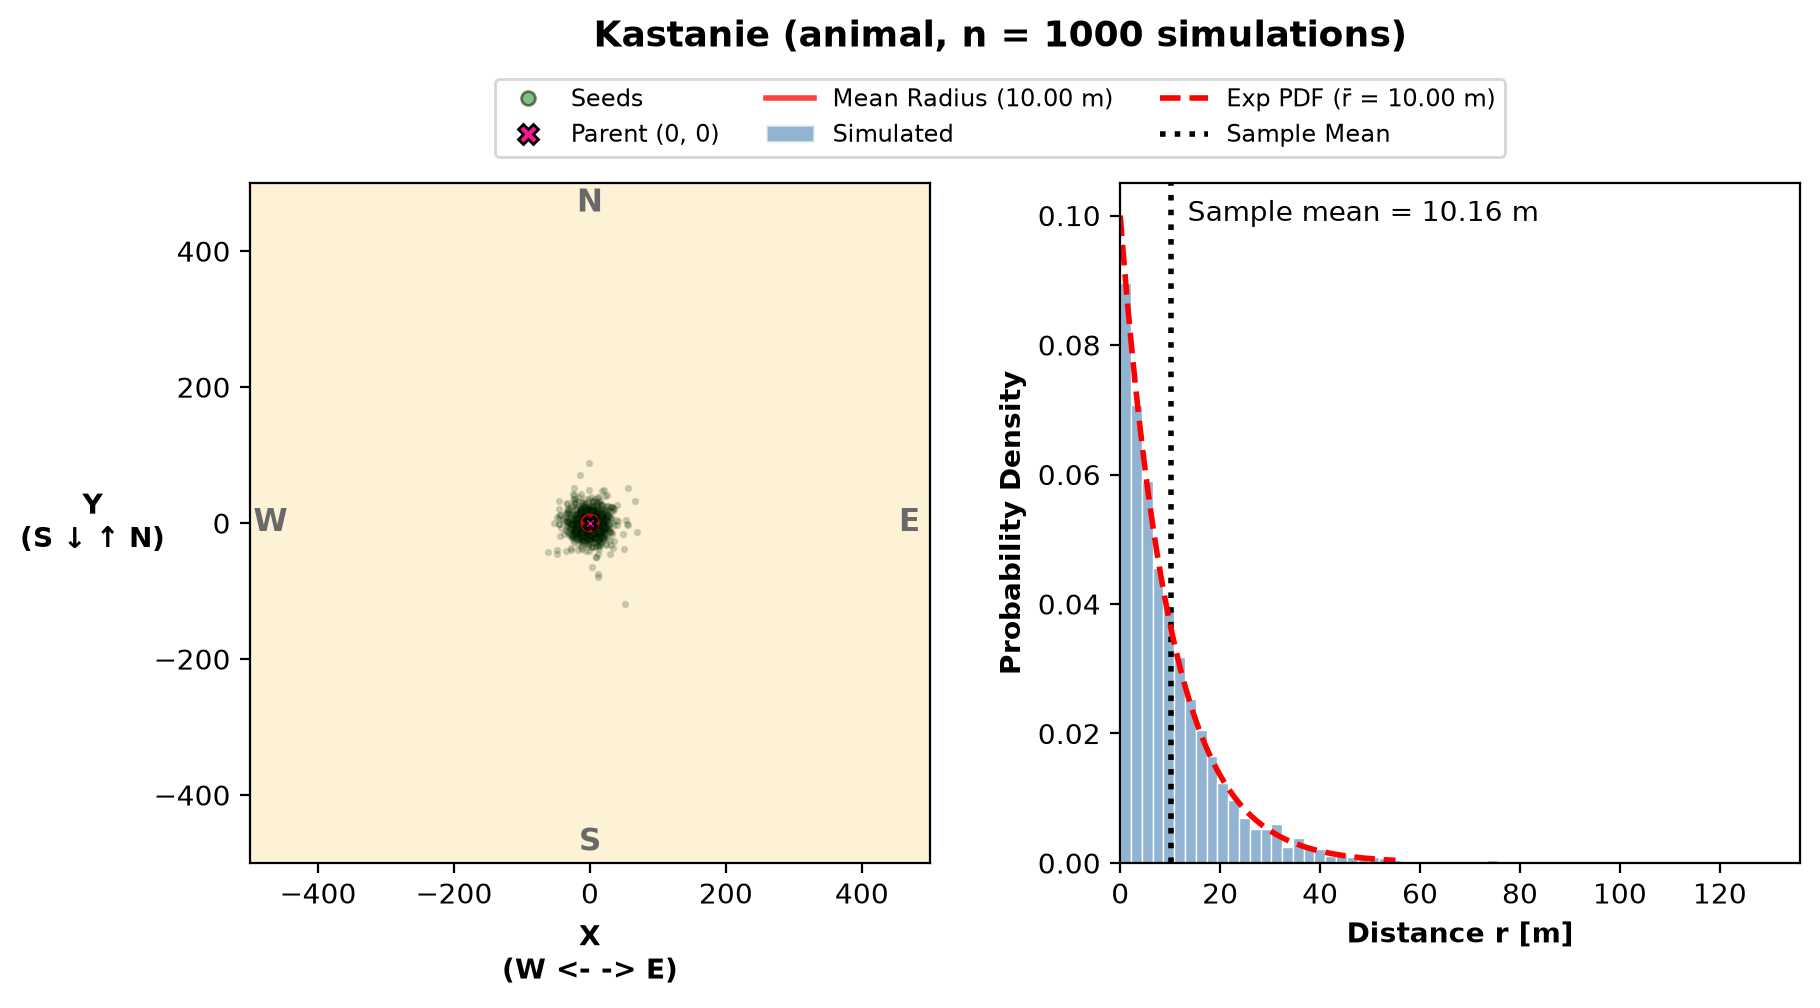
\includegraphics[width=\linewidth]{images/seed_shadow_Kastanie.png}
        \caption{Kastanie (animal)}
        \label{fig:seed_shadow_kastanie}
    \end{subfigure}\hfill
    \begin{subfigure}[b]{0.49\textwidth}
        \centering
        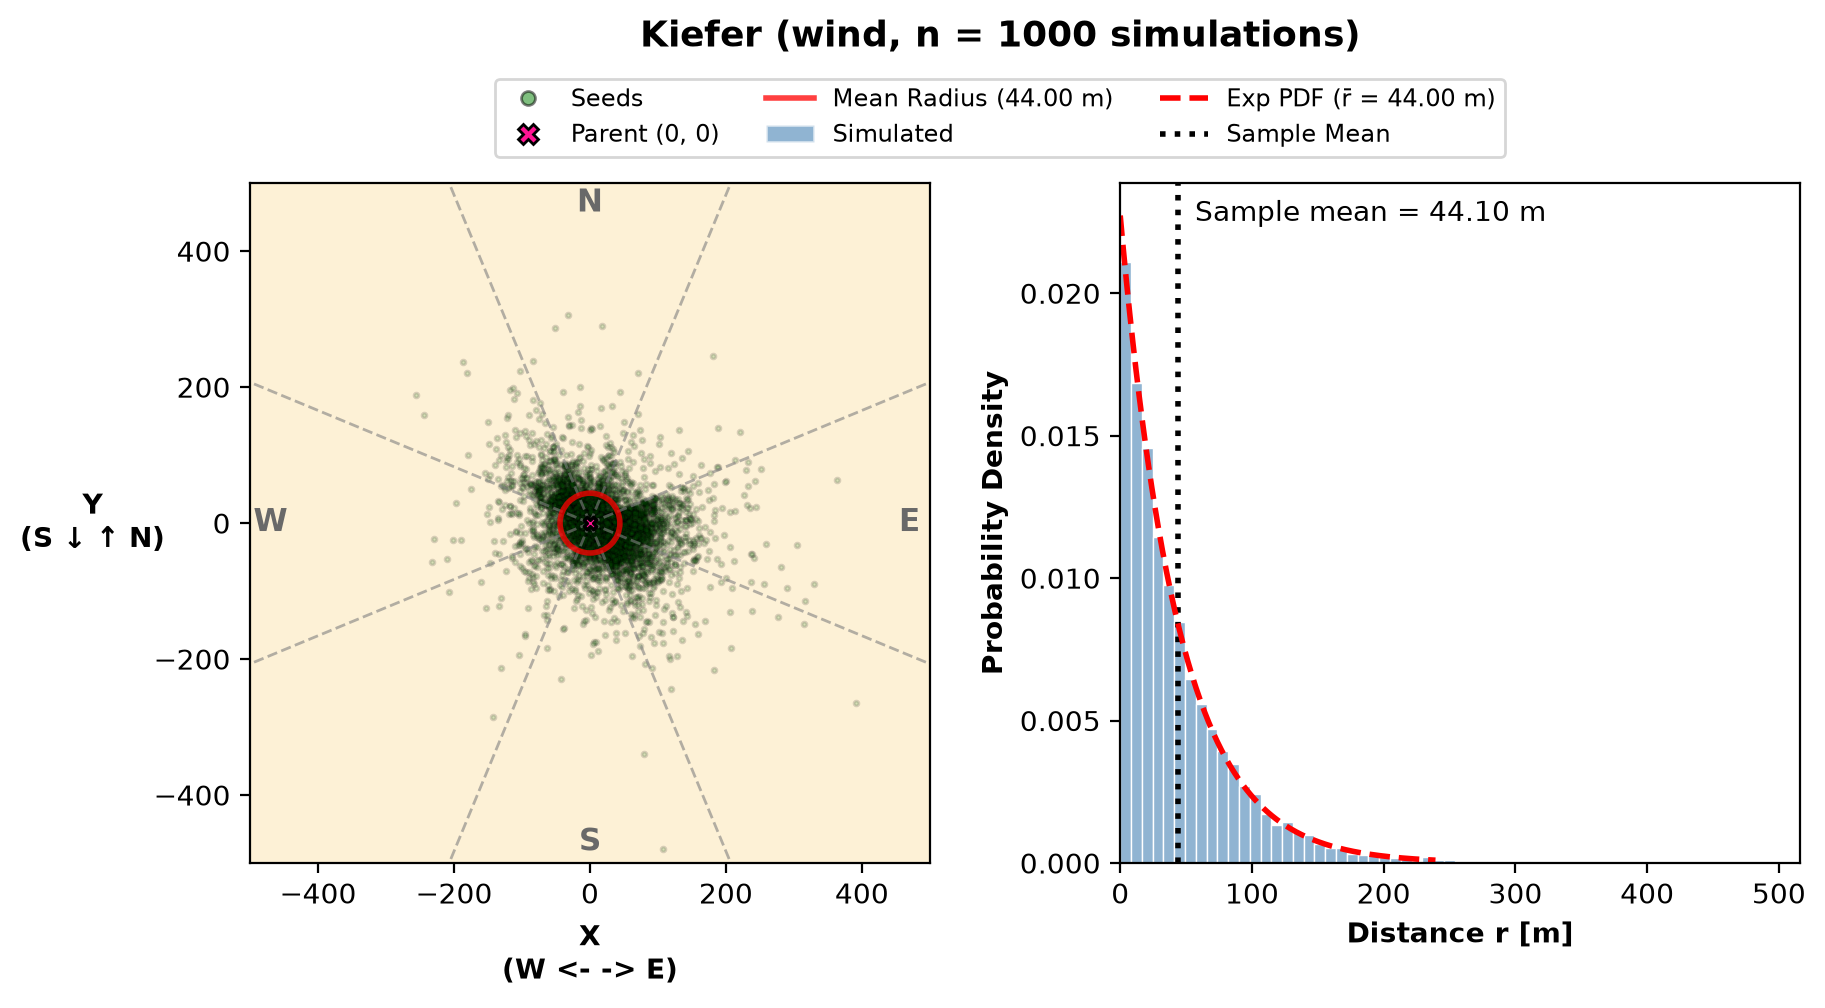
\includegraphics[width=\linewidth]{images/seed_shadow_Kiefer.png}
        \caption{Kiefer (wind)}
        \label{fig:seed_shadow_kiefer}
    \end{subfigure}

    \caption{Simulated seed shadows and radial dispersal distance distributions per species ($k = 4$, $s = 10$, $1000$ simulated years).}
    \label{fig:seed_shadows}
\end{figure}

\clearpage
\begin{figure}[H]
    \ContinuedFloat
    \centering
    \begin{subfigure}[b]{0.49\textwidth}
        \centering
        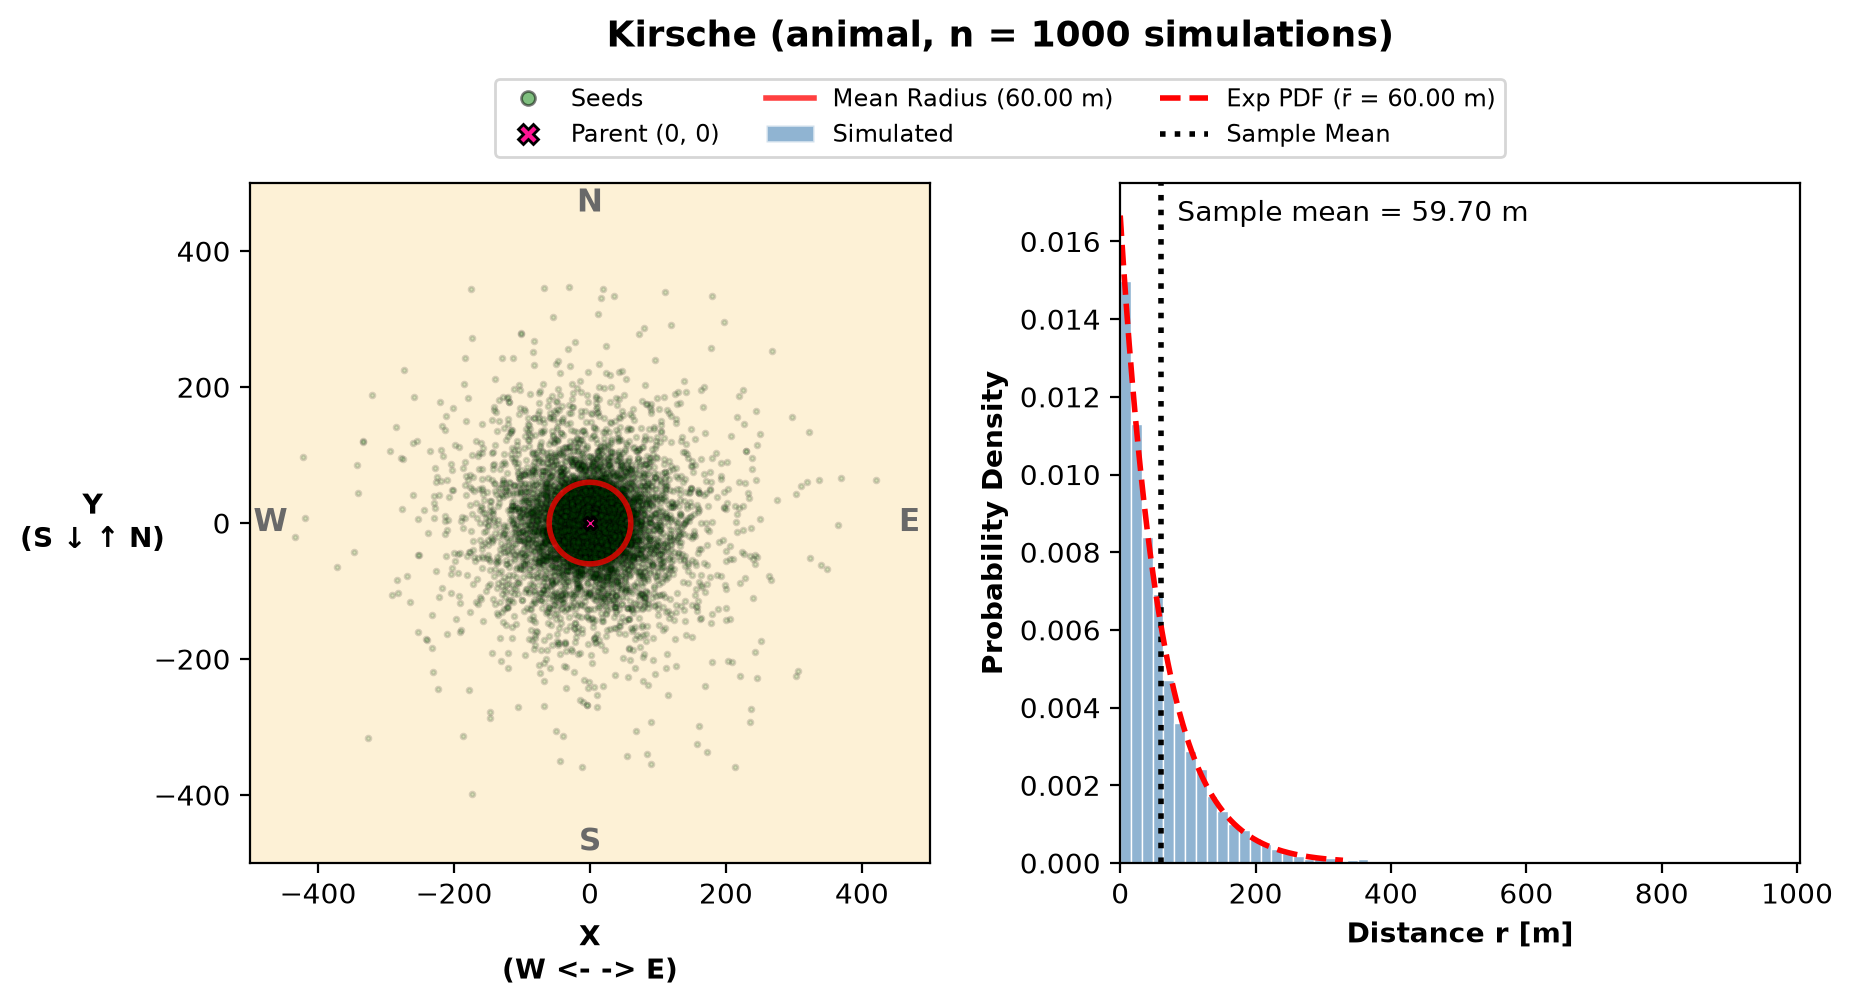
\includegraphics[width=\linewidth]{images/seed_shadow_Kirsche.png}
        \caption{Kirsche (animal)}
        \label{fig:seed_shadow_kirsche}
    \end{subfigure}\hfill
    \begin{subfigure}[b]{0.49\textwidth}
        \centering
        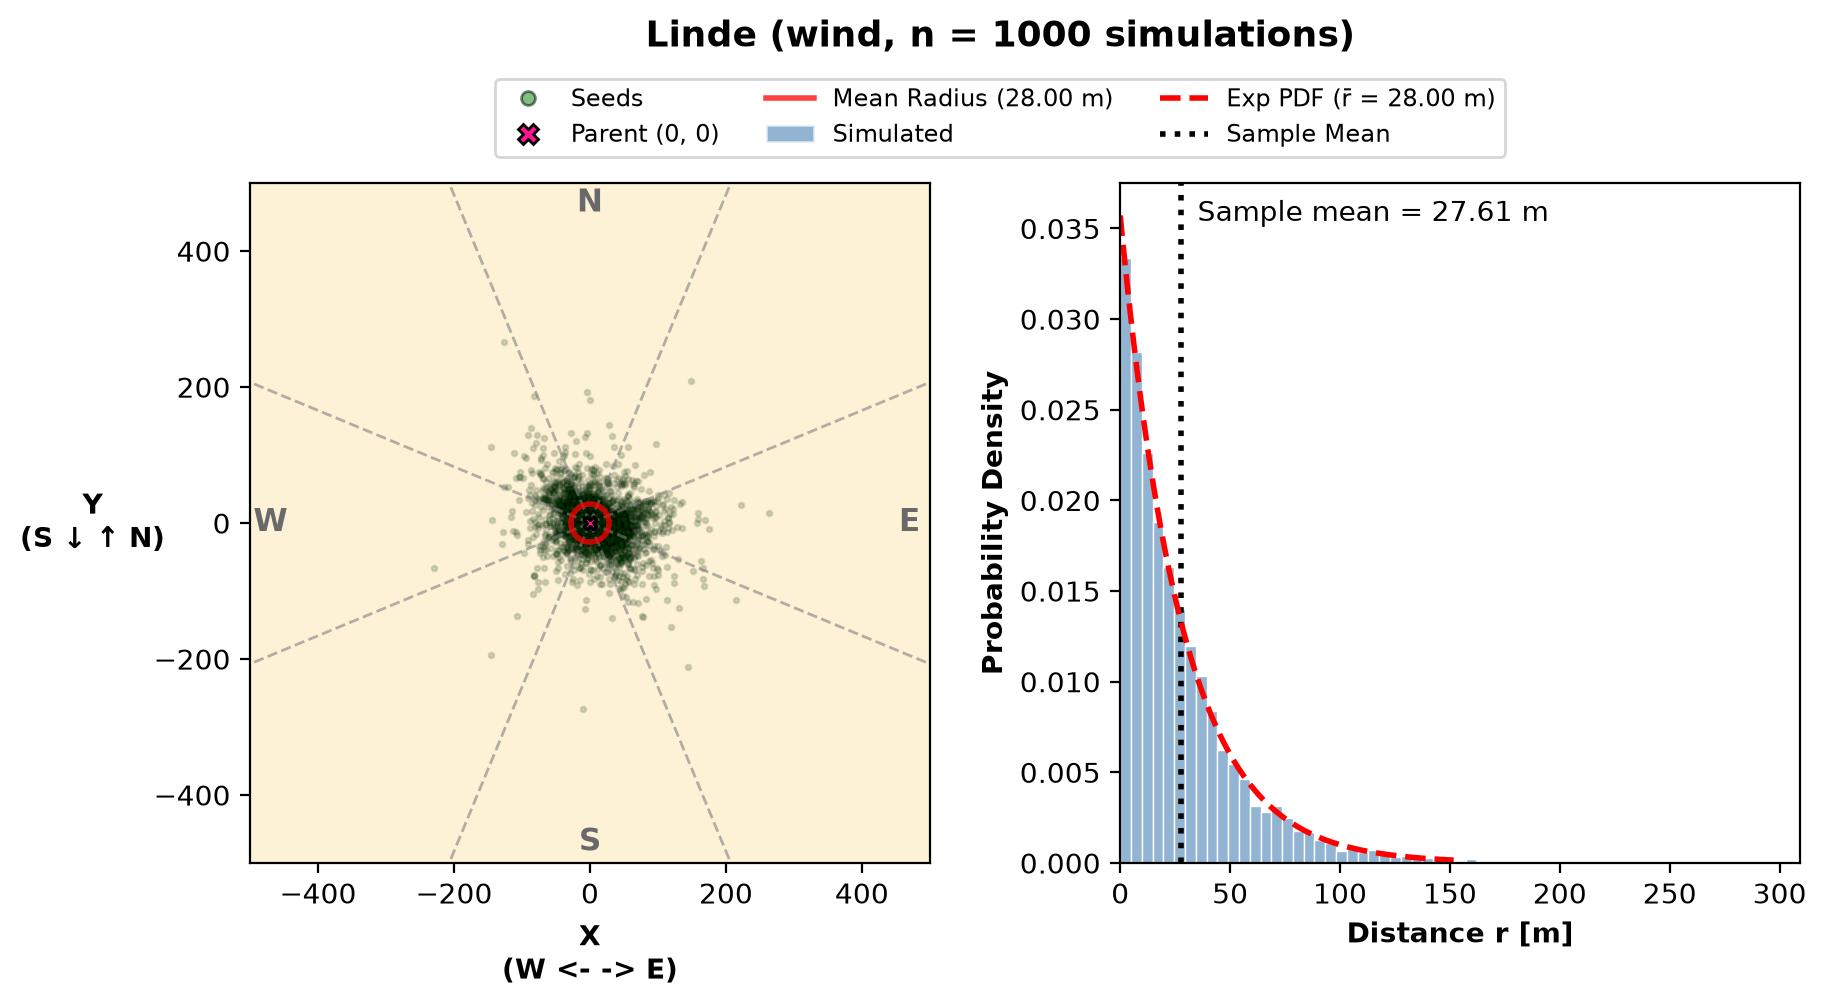
\includegraphics[width=\linewidth]{images/seed_shadow_Linde.png}
        \caption{Linde (wind)}
        \label{fig:seed_shadow_linde}
    \end{subfigure}

    \vspace{0.6em}
    \begin{subfigure}[b]{0.49\textwidth}
        \centering
        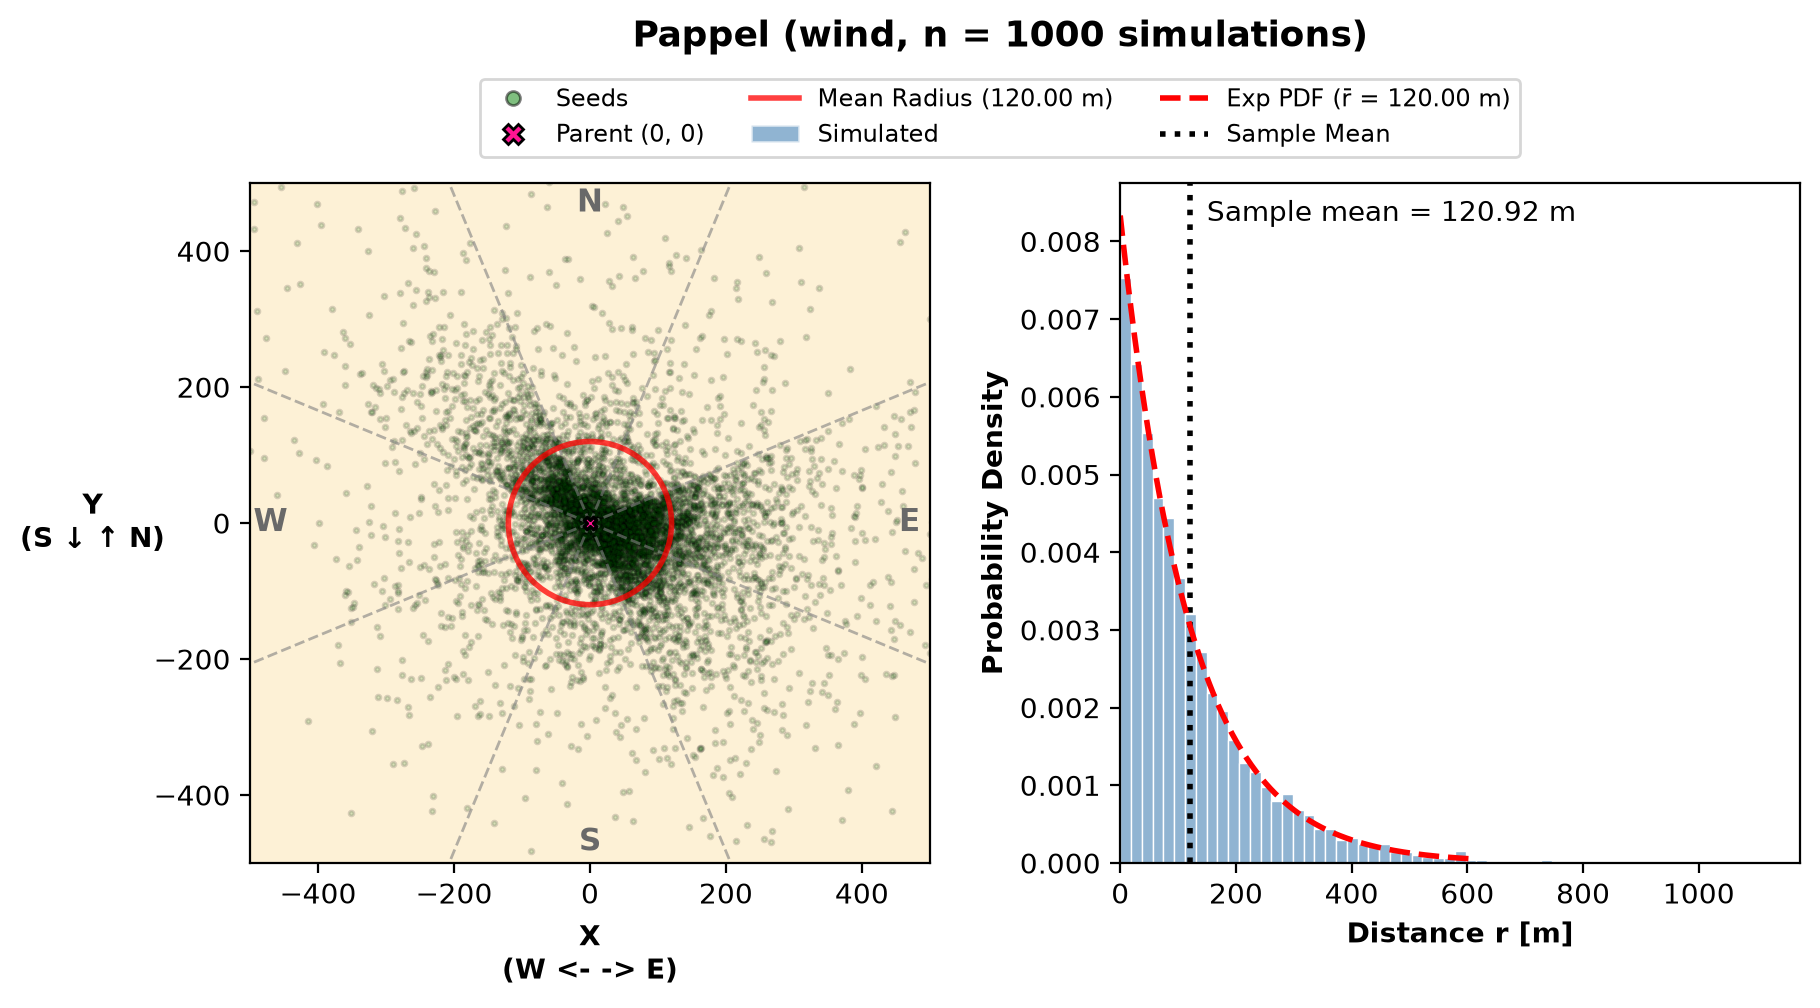
\includegraphics[width=\linewidth]{images/seed_shadow_Pappel.png}
        \caption{Pappel (wind)}
        \label{fig:seed_shadow_pappel}
    \end{subfigure}\hfill
    \begin{subfigure}[b]{0.49\textwidth}
        \centering
        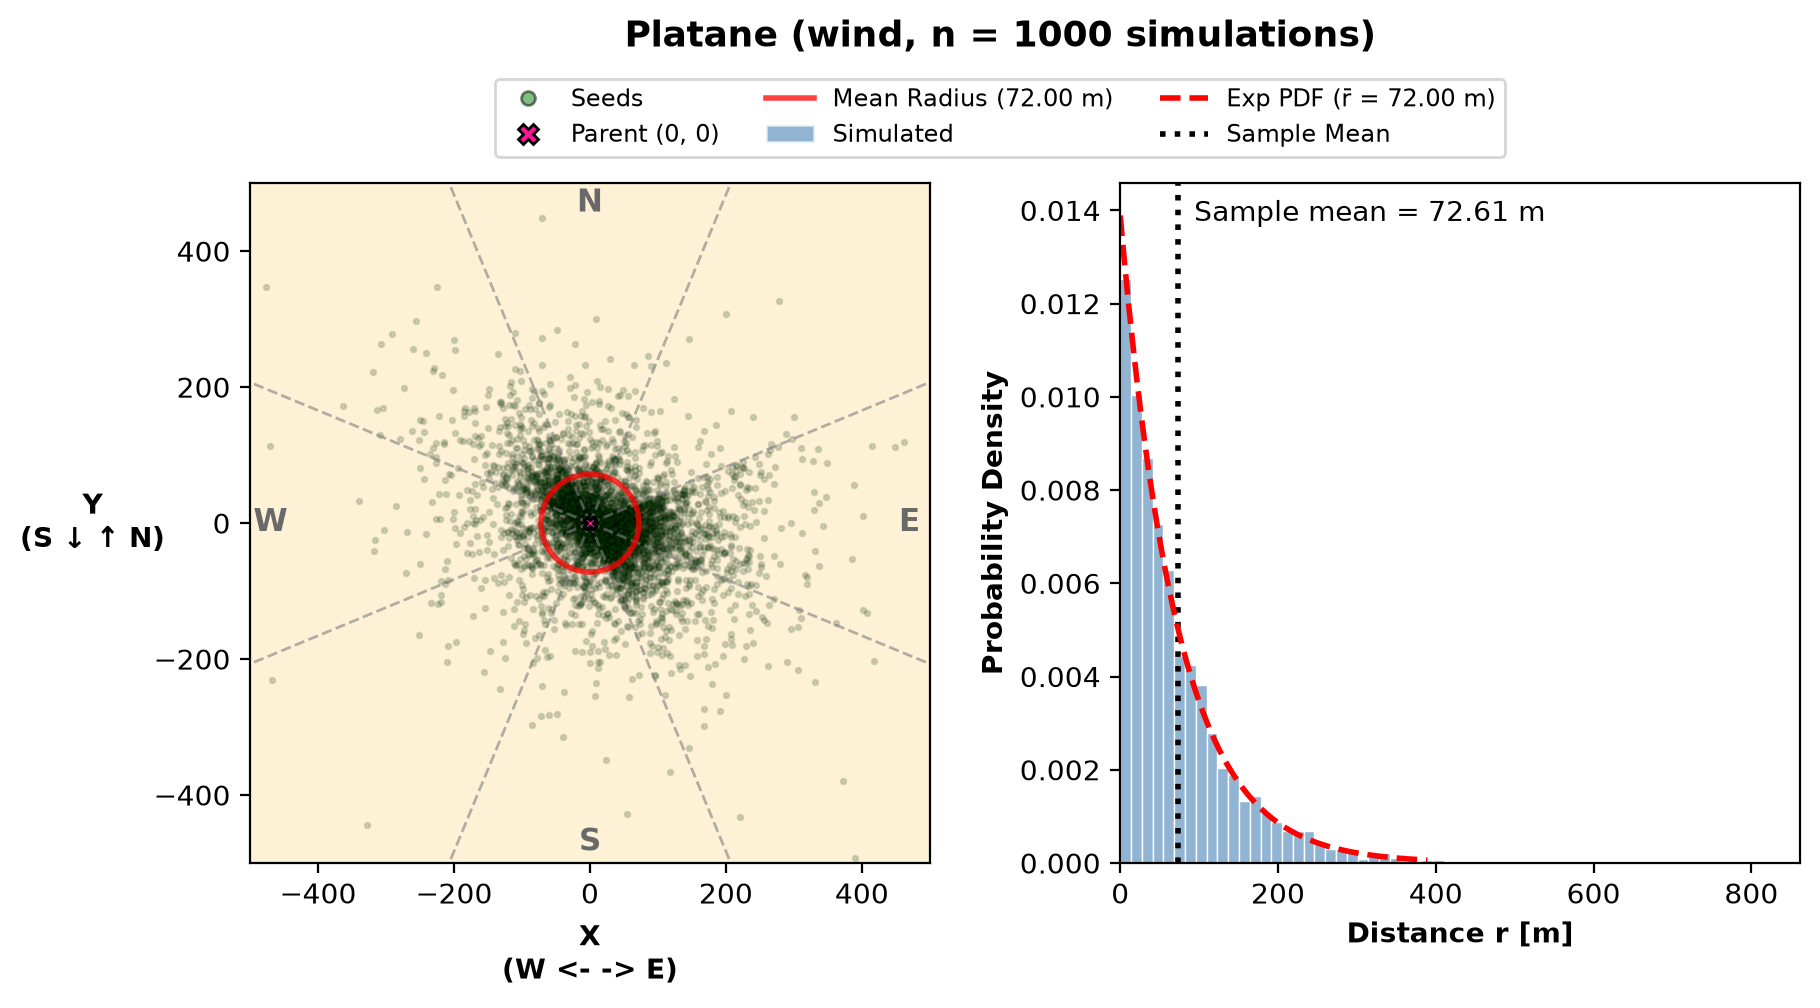
\includegraphics[width=\linewidth]{images/seed_shadow_Platane.png}
        \caption{Platane (wind)}
        \label{fig:seed_shadow_platane}
    \end{subfigure}

    \vspace{0.6em}
    \begin{subfigure}[b]{0.49\textwidth}
        \centering
        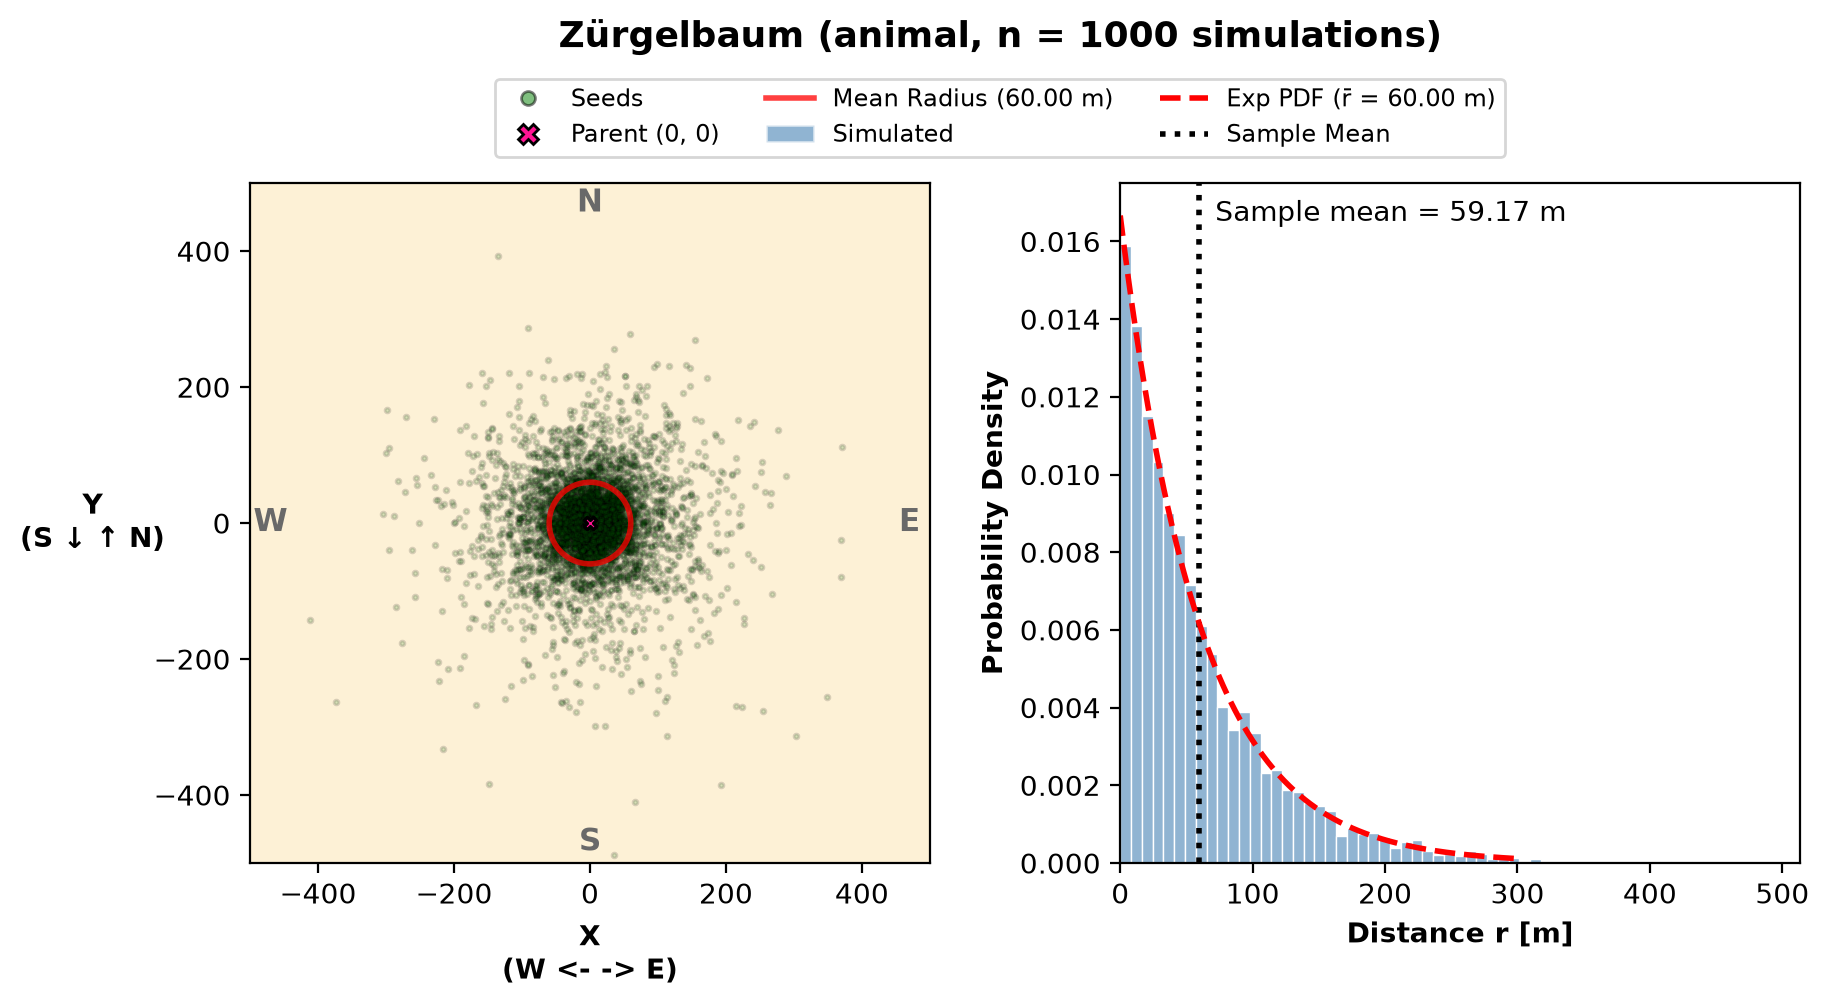
\includegraphics[width=\linewidth]{images/seed_shadow_Zuergelbaum.png}
        \caption{Zürgelbaum (animal)}
        \label{fig:seed_shadow_zuergelbaum}
    \end{subfigure}

    \caption[]{Simulated seed shadows and radial dispersal distance distributions per species (continued).}
\end{figure}

\subsection{Simple forest simulation results}
\todo{add results}

\subsection{Vienna forest simulation results}
\todo{add results}

\section{Discussion}

\paragraph{Summary.}
\todo{Summarize.}

\paragraph{Result Interpretation.}
\todo{Interpret results.}

\paragraph{Conclusion.}
\todo{Conclude.}.

\paragraph{Outlook.}
\todo{Outlook and limitations.}

\section{Statement on the use of AI}
Large language model Gemini was used for a documentation assistant, for refactoring manually created code into clean, modular and pythonic improved code, as an aid for formulating complex mathematical functions. All code files, simulations runs and results were verified by the authors.

\bibliographystyle{plain}
\bibliography{references}
\todo{add if relevant}

\newpage

\appendix
\section{Appendix}
\subsection{Interactive Dashboard Structure}
\todo{Describe interactive app and usage.}

\subsection{Tree species parameters}
The originally defined species parameter table was out of date, and thus the updated (Table~\ref{tab:species_csv}) was provided by the supervisor.
\begin{table}[!ht]
  \centering
  \small
  \csvreader[
    tabular=llrrrrrrrr,
    table head=\toprule
      \textbf{Species} &
      \textbf{Dispersal} &
      $f$ \textbf{[m]} &
      $d_m$ \textbf{[m]} &
      $\p$ &
      $A$ \textbf{[yr]} &
      $T$ \textbf{[yr]} &
      $K$ &
      $L$ \textbf{[yr]} &
      $\ta$ \\ \midrule,
    table foot=\bottomrule,
    late after line=\\
  ]{./tables/tree_species_config.csv}{}{%
    \csvcoli &
    \csvcolii &
    \ifcsvstrequal{\csvcoliii}{}{---}{\csvcoliii} &
    \ifcsvstrequal{\csvcoliv}{}{---}{\csvcoliv} &
    \csvcolv &
    \csvcolvi &
    \csvcolvii &
    \csvcolviii &
    \csvcolix &
    \csvcolx
  }
  \caption{Species parameterization loaded from \texttt{tree\_species\_config.csv}.}
  \label{tab:species_csv}
\end{table}

\end{document}